\chapter{Analiza wymagań aplikacji}
Proces analizy wymagań to kluczowy moment w etapie projektowania aplikacji, który ma na celu usystematyzowanie wymagań klienta, a następnie ich analizę. Jej celem jest sformułowanie zakresu pracy, określenie czasu potrzebnego na wykonanie projektu, a także kosztów, które się z tym wiążą. 
\cite{analiza}

\section{Wymagania funkcjonalne}
Wymagania funkcjonalne definiują w jaki sposób powinna reagować aplikacja bez określania z góry konkretnej technologii, struktury czy też implementacji. Zostały one zaprojektowane w postaci historyjek użytkownika. Jest to bardzo prosta i przystępna forma definiowania wymagań.
\newline
W aplikacji, która jest przedmiotem tej pracy, został wyszczególniony tylko jeden rodzaj użytkownika. Jest to zarejestrowany użytkownik, który wcześniej podał wymagane dane. Ma on dostęp do przeglądania wszystkich przepisów oraz może wykonywać wszystkie możliwe operacje. W aplikacji nie występuje podział na zarejestrowanych i niezarejestrowanych użytkowników, gdyż baza przepisów z założenia ma być budowana przez społeczność, a danie możliwości dodawania nowych receptur byłaby bardzo nierozważna. 
\newline
Poniżej znajdują się historyjki napisane z punktu widzenia użytkownika, które ukazują funkcjonalność aplikacji.
\begin{itemize}
    \item Jako użytkownik chcę na podstawie mojego uwarunkowania fizjologicznego (wzrost, waga, płeć) oraz zadanej ilości posiłków otrzymać listę przepisów, które spełniają moje wymagania.
    \item Jako użytkownik chcę mieć możliwość dodawania nowych przepisów.
    \item Jako użytkownik chcę mieć możliwość dodawania nowych składników, z które można wykorzystać w przepisach.
    \item Jako użytkownik chcę mieć możliwość przeglądania dodanych przeze mnie i innych użytkowników przepisów oraz szczegółów konta.
    \item Jako użytkownik chcę mieć możliwość komentowania przepisów.
    \item Jako użytkownik chcę mieć możliwość oceniania przepisów oraz komentarzy.
    \item Jako użytkownik chcę mieć wyświetlane dane w czytelny i przyjazny sposób.
\end{itemize}

\section{Wymagania niefunkcjonalne}
Wymagania niefunkcjonalne są wymaganiami, które opisują wydajność, niezawodność, bezpieczeństwo oraz właściwości aplikacji.\cite{analiza}
Poniżej znajdują się owe wymagania.
\begin{enumerate}
    \item Aplikacja, będąc aplikacją webową, powinna działać i wyglądać możliwie jak najbardziej podobnie na jak największej ilości obecnie stosowanych nowoczesnych przeglądarkach, tj. Chrome, Firefox, Edge, IE, IE Mobile, Safari, iOS, Android. Powinna też w razie wyjścia nowszych przeglądarek być w łatwy sposób przenoszalna.
    \item Aplikacja powinna przechowywać dane użytkowników w sposób bezpieczny. Tak aby osoby nieupoważnione nie miały do nich dostępu.
    \item Aplikacja powinna uwierzytelniać użytkownika podczas procesu logowania.
    \item Ze względu na jeden typ użytkownika aplikacja nie potrzebuje autoryzacji poprzez role.
    \item W przypadku braku internetu aplikacja nie powinna działać.
    \item Dane niejawne użytkowników, czyli przede wszystkim hasło, powinny być przechowywane w osobnej bazie danych.
\end{enumerate}
\section{Diagram przypadków użycia użytkownika}
Rysunek \ref{fig:use_case} obrazuje diagram przypadków użycia dla użytkownika. Przedstawione przypadki użycia pokrywają główną funkcjonalność aplikacji.

\begin{figure}[h]
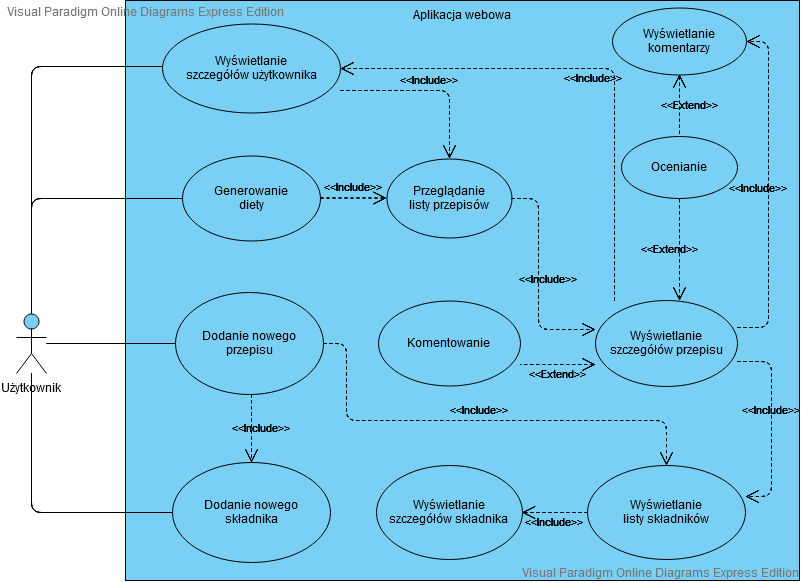
\includegraphics[width=\textwidth]{rys/use-case.png}
\caption{Diagram przypadków użycia}
\label{fig:use_case}
\end{figure}

Poniżej znajduje się krótki opis dla przypadków użycia dla przypadków przedstawionych na rysunku \ref{fig:use_case}.

\begin{enumerate}
    \item Wyświetlanie szczegółów użytkownika\newline
    Przypadek użycia dotyczący wyświetlania informacji dotyczących użytkownika takich jak:
    \begin{itemize}
        \item login,
        \item email,
        \item imię,
        \item nazwisko,
        \item płeć,
        \item data rejestracji,
        \item data ostatniej aktywności.
    \end{itemize}
    
    \item Generowanie diety\newline
    Przypadek użycia dotyczący generowania listy przepisów na podstawie:
    \begin{itemize}
        \item płci,
        \item wzrostu,
        \item wagi.
    \end{itemize}
    
    \item Dodawanie nowego przepisu\newline
    Przypadek użycia dotyczący operacji stworzenia nowego przepisu w systemie. Aby stworzyć przepis należy podać:
    \begin{itemize}
        \item nazwę,
        \item ilość kalorii,
        \item wagę,
        \item opis,
        \item listę składników,
        \item poziom trudności,
        \item szacowany czas przygotowania.
    \end{itemize}
    Utworzenie nowego przepisu w aplikacji jest równoznaczne z dodaniem go w bazie danych.
    
    \item Dodanie nowego składnika\newline
    Przypadek użycia dotyczący operacji stworzenia nowego składnika, który może być później używany w tworzeniu nowych przepisów. Aby stworzyć składnik należy podać:
    \begin{itemize}
        \item nazwę,
        \item opis,
        \item typ składnika,
        \item ilość kalorii na 100 gramów.
    \end{itemize}
    Utworzenie nowego składnika w aplikacji jest równoznaczne z dodaniem go w bazie danych.
    
    \item Przeglądanie listy przepisów\newline
    Przypadek użycia dotyczący wyświetlania listy przepisów. Lista powinna być spójna z szatą graficzną oraz zawierać możliwość paginacji, aby nie była wyświetlana zbyt duża ilość danych. Po wybraniu przepisu z listy powinny zostać wyświetlone jego szczegóły.
    
    \item Komentowanie\newline
    Przypadek użycia dotyczący dodawania komentarzy do przepisu. Wywoływany podczas wyświetlania szczegółów przepisu. Utworzenie nowego komentarza jest równoznaczne z dodaniem go w bazie danych i nie można go później usunąć.
    
    \item Wyświetlanie szczegółów składnika\newline
    Przypadek użycia dotyczący wyświetlania szczegółów składnika, który został wybrany do pokazania przez użytkownika. Powinien zawierać te same dane, które są podawane przy jego wcześniejszym dodawaniu.
    
    \item Wyświetlanie komentarzy\newline
    Przypadek użycia dotyczący wyświetlania komentarzy do przepisu. Komentarze powinny być wyświetlane w prostokątach, a liczba kolumn, w których będą pogrupowane powinna zależeć od wielkości okna przeglądarki. Komentarz powinien zawierać: 
    \begin{itemize}
        \item login użytkownika, który go dodał,
        \item treść,
        \item datę dodania,
        \item ocenę użytkowników.
    \end{itemize}
    
    \item Wyświetlanie szczegółów przepisu\newline
    Przypadek użycia dotyczący wyświetlania szczegółów przepisu, który mógł zostać wygenerowany i wybrany jako jeden z elementów składowych diety albo wybrany jako przepis dodany przez wcześniej oglądanego użytkownika. Powinien zawierać te same dane, które są podawane przy jego wcześniejszym dodawaniu oraz dodatkowo ocenę użytkowników.

    \item Ocenianie\newline
    Przypadek użycia dotyczący ocenianiu przez społeczność przepisów oraz komentarzy. Polega na oddaniu głosu pozytywnego lub negatywnego. System powinien nie zezwalać użytkownikowi na powtórne ocenienie tego samego elementu.
    
    \item Wyświetlanie listy składników\newline
    Przypadek użycia dotyczący wyświetlania listy składników. Lista powinna być spójna z szatą graficzną oraz zawierać możliwość paginacji, aby nie była wyświetlana zbyt duża ilość danych. Po wybraniu składnika z listy powinny zostać wyświetlone jego szczegóły.
\end{enumerate}